\subsection{三类典型工作负载特征}

本文采用"遥操作采集—服务器训练—边缘推理"的标准流程构建实验数据集。
数据采集阶段，操作者手持 leader 臂进行示教，SO-101 follower 臂实时同步复现动作，
LeRobot 同步记录所有关节角度与两路摄像头图像，形成结构化 episode 文件。
每类任务录制 50 个 episode，三类共 150 个 episode。
训练阶段，将数据集传至配备 GPU 的服务器，调用 LeRobot \texttt{train} 命令以 ACT 策略进行监督学习，
生成模型权重文件。推理阶段，将权重部署至树莓派5，
由 \texttt{record.py} 加载 policy 执行在线闭环推理，实验数据均在此阶段采集。

三类任务按操作复杂度从低到高设计，以考察不同难度下系统的推理行为是否存在差异：

\begin{center}
\begin{tabular}{clp{0.5\textwidth}}
  \toprule
  难度 & 任务 & 描述 \\
  \midrule
  低 & 抓取（Grasp） & 场景中放置 1 个瓶子，机械臂识别并完成抓取；目标唯一，动作路径固定 \\
  中 & 推倒（Push）  & 场景中放置 2 个瓶子，需识别指定目标并将其推倒；引入目标选择判断 \\
  高 & 分类（Sort）  & 场景中放置 3 个瓶子，需按指定顺序逐一抓取并分类摆放；需要长程规划与多步序列操作 \\
  \bottomrule
\end{tabular}
\end{center}

三类任务统一使用树莓派5、ACT（\texttt{chunk\_size=100}）、目标帧率 30\,fps，
每类任务取 $n=50$ 个 episode 的统计结果作为基准画像，
只比较各阶段时间占比，而不把 episode 绝对时长差异混入分析。

\begin{figure}[H]
  \centering
  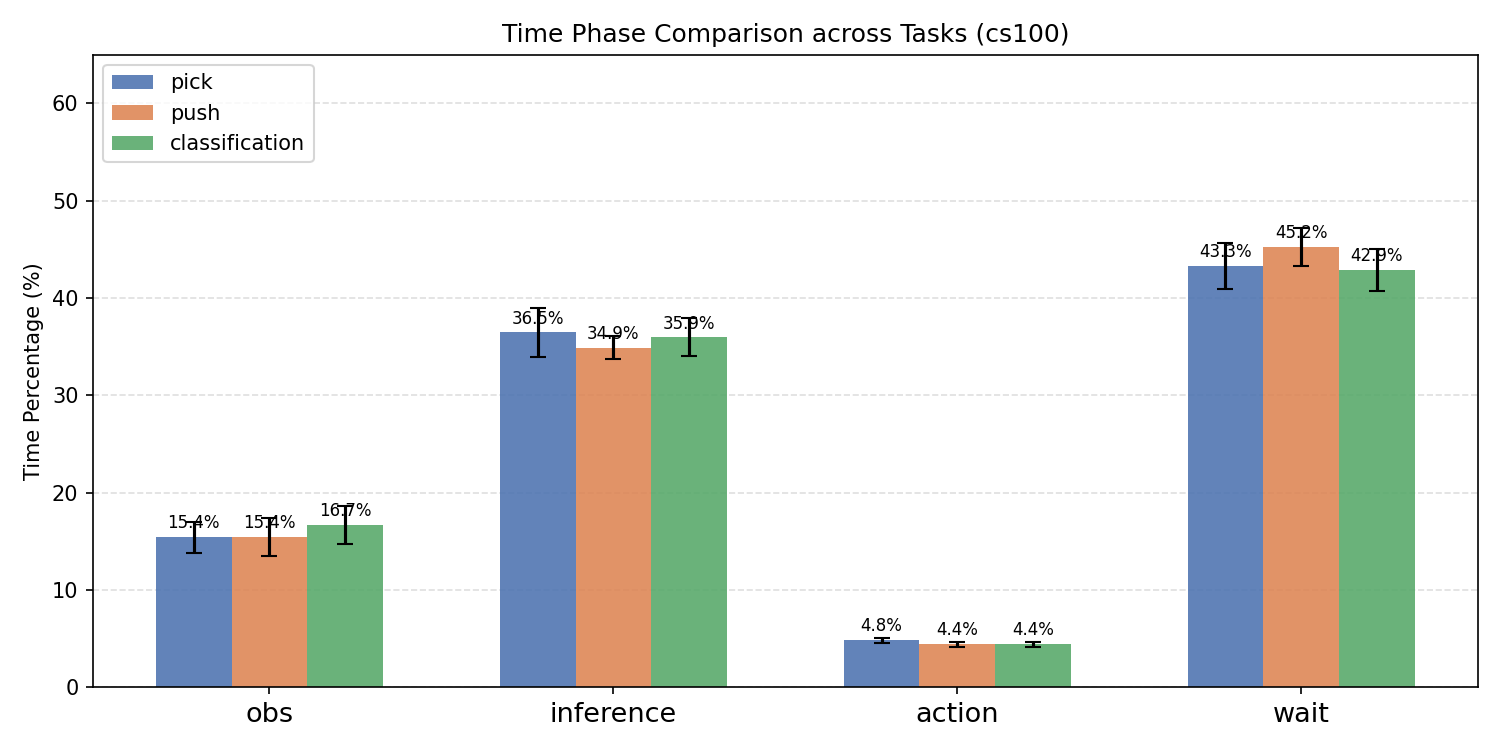
\includegraphics[width=0.92\textwidth]{../实验/02_三类任务工作负载对比/cs100_task_comparison.png}
  \caption{三类任务在 \texttt{chunk\_size=100} 下的阶段时间占比对比}
  \label{fig:cs100-task-comparison}
\end{figure}

图~\ref{fig:cs100-task-comparison} 的主要现象有三点。
第一，三类任务的推理占比都集中在 35\%--36\% 左右，
说明在模型结构、\texttt{chunk\_size} 和输入配置相同的情况下，
ACT 单次推理开销主要由模型本身决定，而不是由抓取、推倒、分类这些任务语义决定。
第二，推倒任务的 \texttt{wait\_pct} 最高，达到 45.2\%，
比抓取和分类高约 2 个百分点；这更像是动作行程和执行节奏造成的等待增加，
而不是推理侧变慢。
第三，\texttt{obs\_pct} 和 \texttt{action\_pct} 在三类任务之间变化很小，
说明相机读取、舵机状态读取以及舵机写入在当前实验设置下更接近固定开销。

因此，后续性能分析不把三类任务视为三种完全不同的软件路径，
而是把它们看作同一 LeRobot 推理循环在不同动作负载下的表现。
抓取和分类更接近基准工作负载；推倒任务由于等待占比最高，
更适合用来观察执行节奏和 \texttt{chunk\_size} 对整体帧率的影响。

\src{实验/02\_三类任务工作负载对比/cs100\_task\_comparison.md}
